\documentclass[a4paper]{article}

\usepackage{afterpage}
\usepackage{bold-extra}
\usepackage{color}
\usepackage{float}
\usepackage{graphicx}
\usepackage{listings}
\usepackage{subfigure}

%%%%%%%%%%%%%%%
%%% Colours %%%
%%%%%%%%%%%%%%%

\definecolor{darkgreen}{rgb}{0, 0.6, 0}
\definecolor{lightgrey}{gray}{0.9}

%%%%%%%%%%%
% Figures %
%%%%%%%%%%%

% Define shorter ways to include individual images
\newcommand{\stufig}[4]						% images with default placement
{
	\begin{figure}
	\begin{center}
		\includegraphics[#1]{#2}
		\caption{#3}
		\label{#4}
	\end{center}
	\end{figure}
}

\newcommand{\stufigex}[5]					% images with specified placement
{
	\begin{figure}[#5]
	\begin{center}
		\includegraphics[#1]{#2}
		\caption{#3}
		\label{#4}
	\end{center}
	\end{figure}
}

\newcommand{\stufigexx}[5]				% full-width images with specified placement
{
	\begin{figure*}[#5]
	\begin{center}
		\includegraphics[#1]{#2}
		\caption{#3}
		\label{#4}
	\end{center}
	\end{figure*}
}

% Define the stusubfig environment
\newenvironment{stusubfig}[1]
{
	\begin{figure*}[#1]
	\begin{center}
}
{
	\end{center}
	\end{figure*}
}

%%%%%%%%%%%%%%%%%
% Code Listings %
%%%%%%%%%%%%%%%%%

% Create a new type of float (called a stulisting) for listings
\floatstyle{ruled}
\newfloat{stulisting}{thp}{lop}
\floatname{stulisting}{Listing}

% Setup before using the listings package
\renewcommand{\lstlistingname}{\textbf{Listing}}
\def\thelstlisting{\textbf{\arabic{lstlisting}}}

\lstdefinelanguage{Pseudocode}{
morekeywords={and,assert,break,case,continue,default,down,each,else,for,function,if,not,null,or,rangeswitch,ref,return,switch,then,this,throw,to,up,var,while},
sensitive=true,
morecomment=[l]{//},
morecomment=[s]{/*}{*/}
}

\lstdefinestyle{Default}{
abovecaptionskip=0.5cm,
basicstyle=\scriptsize\ttfamily,
belowcaptionskip=0.5cm,
belowskip=0.5cm,
columns=fixed,
%commentstyle=\color{darkgreen},
commentstyle=\textit, % changed from the thesis (green text looks unprofessional in a journal paper)
language=Pseudocode,
%numbers=left,
numbers=none, % changed from the thesis (line numbers are less relevant here)
numbersep=5pt,
numberstyle=\tiny,
mathescape=true,
showstringspaces=false,
stepnumber=1,
tabsize=4
}

\lstdefinestyle{Snippet}{
abovecaptionskip=0.5cm,
aboveskip=0.5cm,
basicstyle=\small\ttfamily,
belowcaptionskip=0.5cm,
belowskip=0.5cm,
columns=fixed,
commentstyle=\color{darkgreen},
frame=lines,
keywordstyle=\small\bfseries,
language=Pseudocode,
numbers=none,
mathescape=true,
showstringspaces=false,
stepnumber=1,
tabsize=4
}

% For C++ function prototypes
\lstdefinestyle{Prototype}{
abovecaptionskip=0.5cm,
basicstyle=\small\ttfamily,
belowcaptionskip=0.5cm,
belowskip=0.5cm,
columns=fixed,
commentstyle=\color{darkgreen},
language=C++,
numbers=none,
mathescape=true,
showstringspaces=false,
stepnumber=1,
tabsize=4
}

%%%%%%%%%%%%%%%%%
% Main Document %
%%%%%%%%%%%%%%%%%

\begin{document}

\title{Two Tree-Based Algorithms for the Waterfall}
\author{S M Golodetz, C Nicholls, I D Voiculescu and S A Cameron}
\date{Draft of \today}
\maketitle

\begin{abstract}
\noindent TODO
\end{abstract}

%#####################
\section{Introduction}
%#####################

TODO: \cite{golodetz11}

%###################
\section{Background}
%###################

\subsection{The Watershed Transform}

TODO

\subsection{The Waterfall Transform}

TODO

\subsection{Marcotegui's Algorithm}

TODO

%############################
\section{Nicholls' Algorithm}
%############################

TODO

%#############################
\section{Golodetz's Algorithm}
%#############################

TODO

%###################
\section{Comparison}
%###################

\subsection{Method}

TODO

\subsection{Results}

TODO

%###################
\section{Discussion}
%###################

TODO

%####################
\section{Conclusions}
%####################

TODO

%---
\begin{stusubfig}{p}
	\subfigure[Before rooting the MST]
	{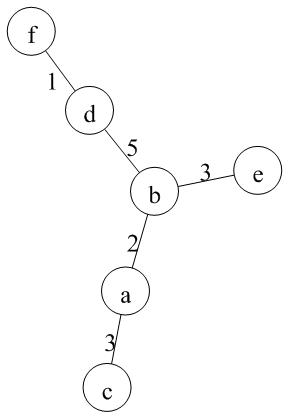
\includegraphics[height=6cm]{segmentation-waterfall-nicholls-root-before.png}}%
	%
	\hspace{4mm}%
	%
	\subfigure[After rooting it]
	{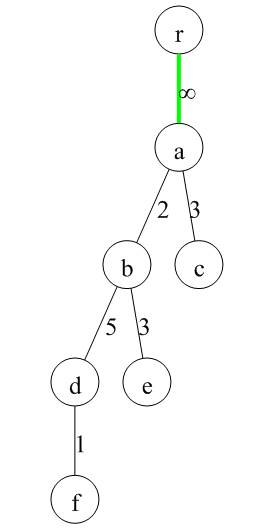
\includegraphics[height=6cm]{segmentation-waterfall-nicholls-root-after.png}}%
\caption{Nicholls' algorithm starts by picking a node at which to root the MST}% and adding a dummy root edge above the chosen root}
\label{fig:segmentation-waterfall-nicholls-root}
\end{stusubfig}
%---

%---
\begin{stusubfig}{p}
	\subfigure[The considered edge is not the unique lowest edge]
	{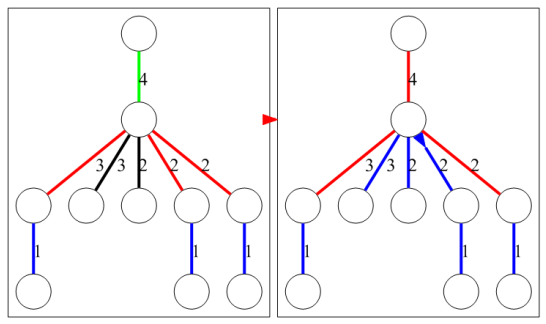
\includegraphics[height=5cm]{segmentation-waterfall-nicholls-cases-a.png}}%
	%
	\hspace{4mm}%
	%
	\subfigure[The considered edge is the unique lowest edge]
	{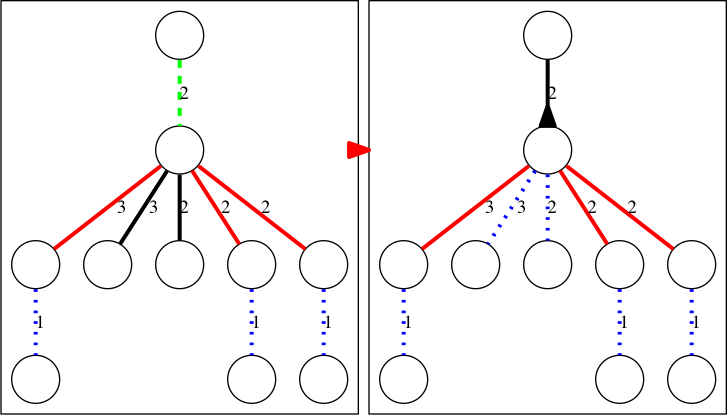
\includegraphics[height=5cm]{segmentation-waterfall-nicholls-cases-b.png}}%
\caption[Case analysis for the recursive step of Nicholls' algorithm]{Case analysis for the recursive step of Nicholls' algorithm: black edges are non-guards, red edges are guards, blue edges are those which have been elided and the green edge is the one under active consideration. The arrow (on the node) indicates the direction in which the algorithm presumes water to flow.}
\label{fig:segmentation-waterfall-nicholls-cases}
\end{stusubfig}
%---

%---
\begin{stusubfig}{p}
	\subfigure[Level 7]{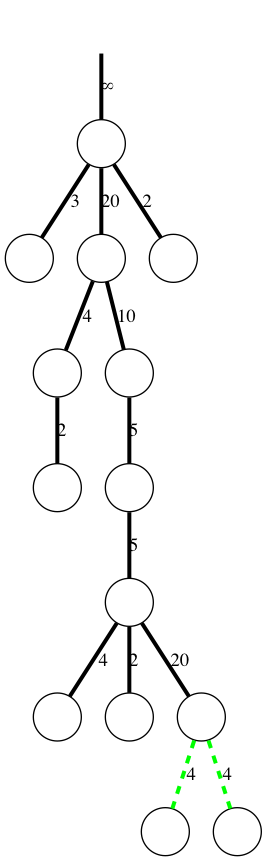
\includegraphics[width=.17\linewidth]{segmentation-waterfall-nicholls-example-a.png}}%
	\hspace{4mm}%
	\subfigure[Level 6]{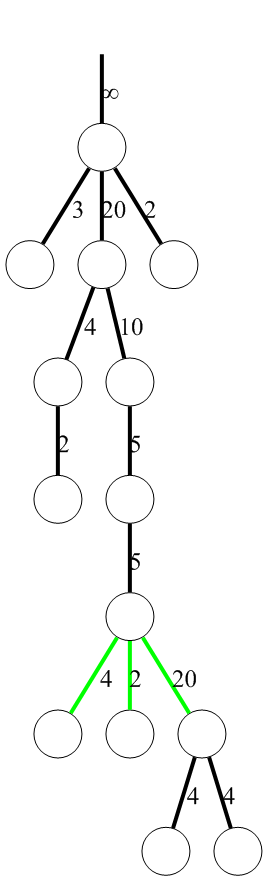
\includegraphics[width=.17\linewidth]{segmentation-waterfall-nicholls-example-b.png}}%
	\hspace{4mm}%
	\subfigure[Level 5]{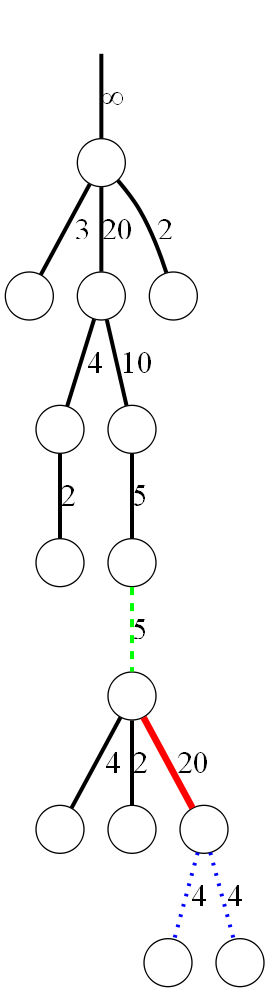
\includegraphics[width=.17\linewidth]{segmentation-waterfall-nicholls-example-c.png}}%
	\hspace{4mm}%
	\subfigure[Level 4]{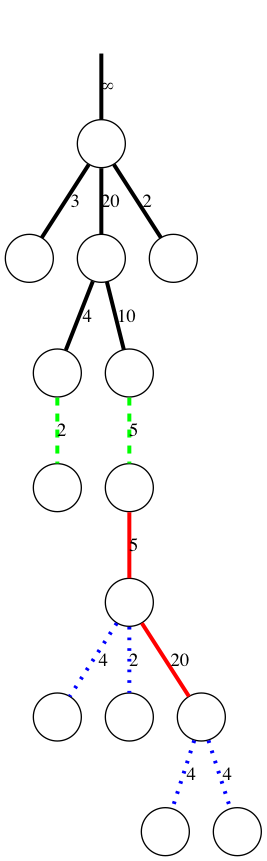
\includegraphics[width=.17\linewidth]{segmentation-waterfall-nicholls-example-d.png}}%
	\\
	\subfigure[Level 3]{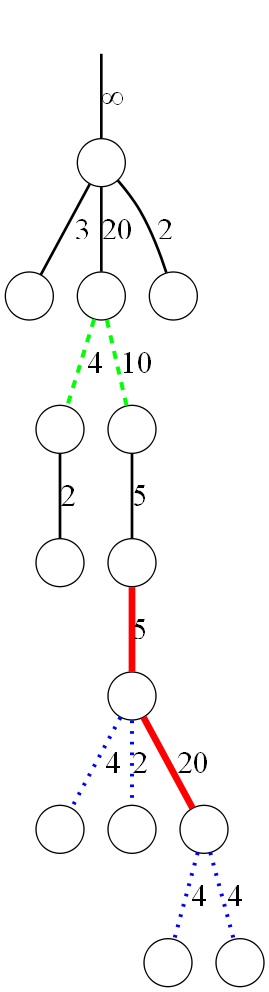
\includegraphics[width=.17\linewidth]{segmentation-waterfall-nicholls-example-e.png}}%
	\hspace{4mm}%
	\subfigure[Level 2]{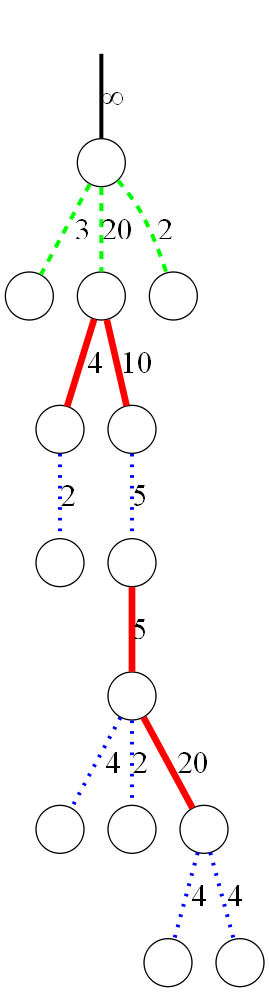
\includegraphics[width=.17\linewidth]{segmentation-waterfall-nicholls-example-f.png}}%
	\hspace{4mm}%
	\subfigure[Level 1]{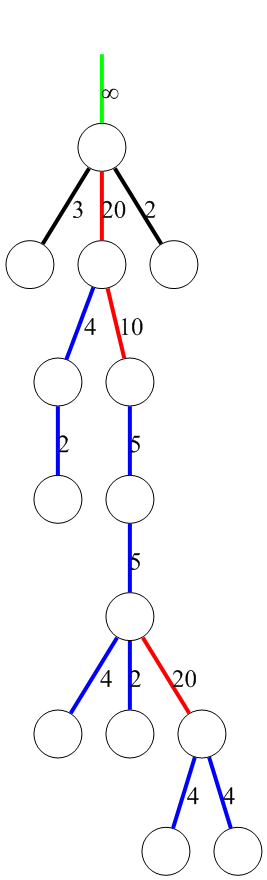
\includegraphics[width=.17\linewidth]{segmentation-waterfall-nicholls-example-g.png}}%
	\hspace{4mm}%
	\subfigure[Result]{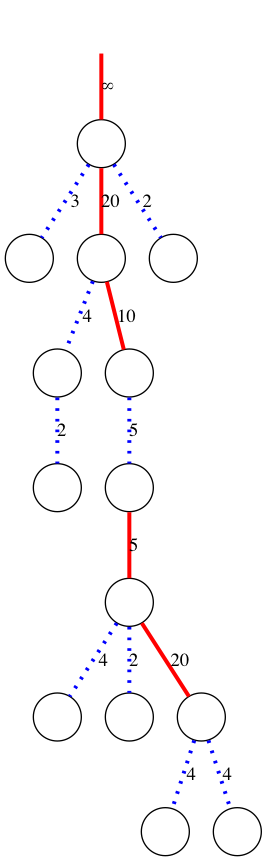
\includegraphics[width=.17\linewidth]{segmentation-waterfall-nicholls-example-h.png}}%
\caption[Nicholls' algorithm in action]{Nicholls' algorithm in action (considering all the edges in each level at a time for space reasons): black edges are non-guards, red edges are guards, blue edges are those which have been elided and green edges are ones under active consideration.}
\label{fig:segmentation-waterfall-nicholls-example}
\end{stusubfig}
%---

%---
\begin{stusubfig}{p}
	\subfigure[UI/UI]{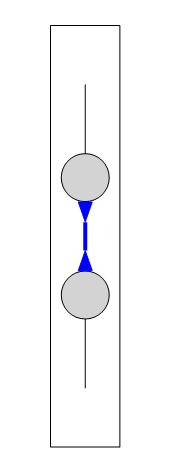
\includegraphics[height=5cm]{segmentation-waterfall-smg-mergecases-uiui.png}}%
	\hspace{4mm}
	\subfigure[UI/UO]{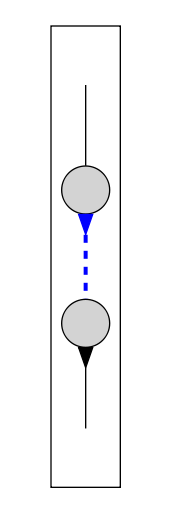
\includegraphics[height=5cm]{segmentation-waterfall-smg-mergecases-uiuo.png}}%
	\hspace{4mm}
	\subfigure[UO/AO]{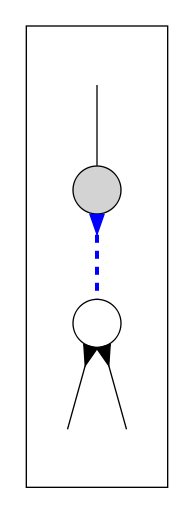
\includegraphics[height=5cm]{segmentation-waterfall-smg-mergecases-uiao.png}}%
	\hspace{4mm}
	\subfigure[UI/NF]{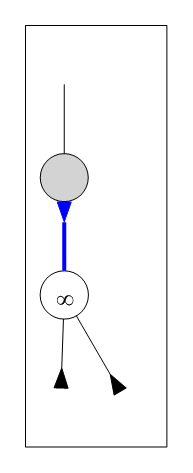
\includegraphics[height=5cm]{segmentation-waterfall-smg-mergecases-uinf.png}}%
	\hspace{4mm}
	\subfigure[NF/NF]{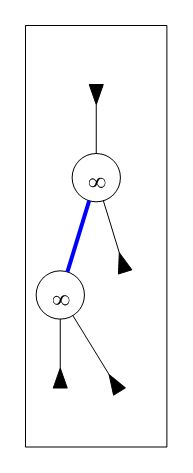
\includegraphics[height=5cm]{segmentation-waterfall-smg-mergecases-nfnf.png}}%
	\\
	\subfigure[UO/UO]{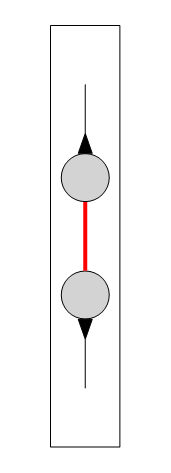
\includegraphics[height=5cm]{segmentation-waterfall-smg-mergecases-uouo.png}}%
	\hspace{4mm}
	\subfigure[UO/AI]{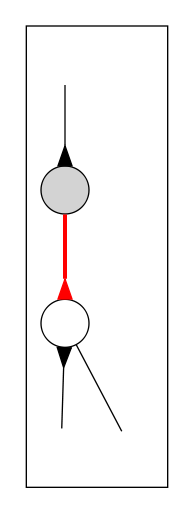
\includegraphics[height=5cm]{segmentation-waterfall-smg-mergecases-uoai.png}}%
	\hspace{4mm}
	\subfigure[UO/AO]{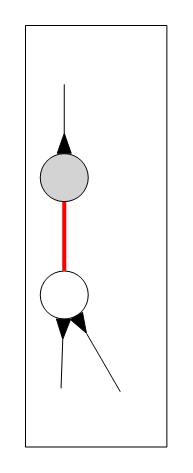
\includegraphics[height=5cm]{segmentation-waterfall-smg-mergecases-uoao.png}}%
	\hspace{4mm}
	\subfigure[UO/NF]{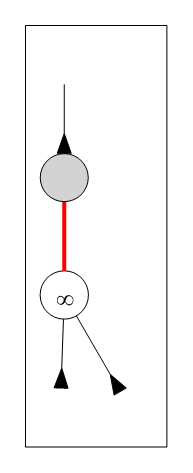
\includegraphics[height=5cm]{segmentation-waterfall-smg-mergecases-uonf.png}}%
	\\
	\subfigure[AO/AI]{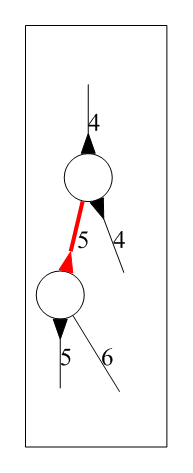
\includegraphics[height=5cm]{segmentation-waterfall-smg-mergecases-aoai.png}}%
	\hspace{4mm}
	\subfigure[AO/AO]{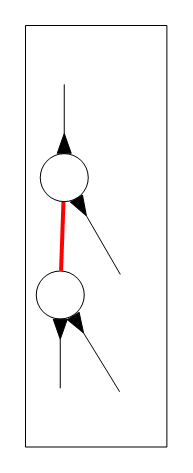
\includegraphics[height=5cm]{segmentation-waterfall-smg-mergecases-aoao.png}}%
	\hspace{4mm}
	\subfigure[NF/AI]{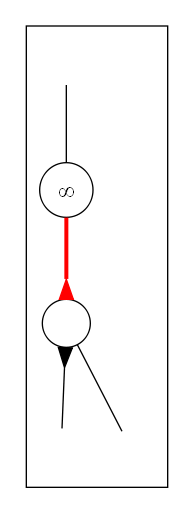
\includegraphics[height=5cm]{segmentation-waterfall-smg-mergecases-nfai.png}}%
	\hspace{4mm}
	\subfigure[NF/AO]{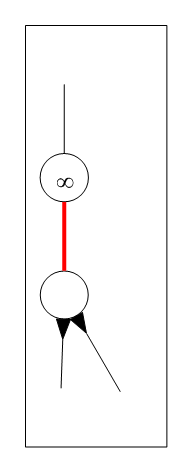
\includegraphics[height=5cm]{segmentation-waterfall-smg-mergecases-nfao.png}}%
\caption[Case analysis for the edge elision step of my waterfall algorithm]{Case analysis for the edge elision step of my waterfall algorithm (a blue edge indicates that the edge would be elided; a red edge indicates that it wouldn't). The labels are AI = ambiguous in, AO = ambiguous out, NF = no flow, UI = unambiguous in and UO = unambiguous out.}
\label{fig:segmentation-waterfall-smg-mergecases}
\end{stusubfig}
%---

%---
\begin{stusubfig}{p}
	\subfigure[The node has a unique path of steepest descent down a child edge]
	{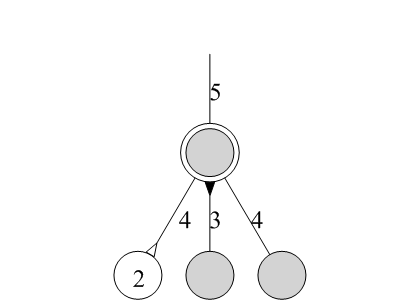
\includegraphics[width=.35\linewidth]{segmentation-waterfall-smg-pass1cases-a.png}}%
	%
	\hspace{4mm}%
	%
	\subfigure[The node has a unique path of steepest descent up the parent edge]
	{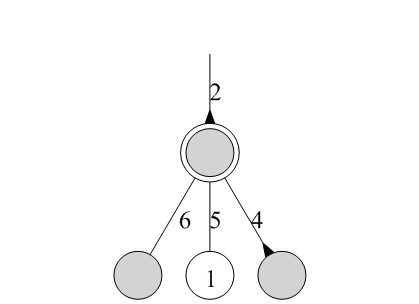
\includegraphics[width=.35\linewidth]{segmentation-waterfall-smg-pass1cases-b.png}}%
	%
	\hspace{4mm}%
	%
	\subfigure[The node has more than one path of steepest descent (and the parent edge is not a possible path of steepest descent)]
	{\hspace{8mm}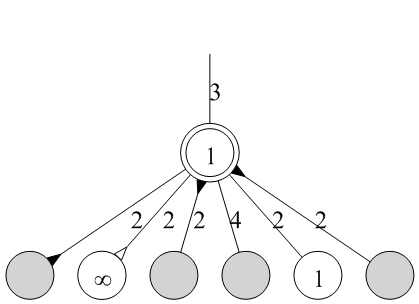
\includegraphics[width=.35\linewidth]{segmentation-waterfall-smg-pass1cases-c.png}\hspace{8mm}}%
	%
	\hspace{4mm}%
	%
	\subfigure[The node has more than one \emph{downwards} path of steepest descent (but the parent edge still needs to be considered)]
	{\hspace{8mm}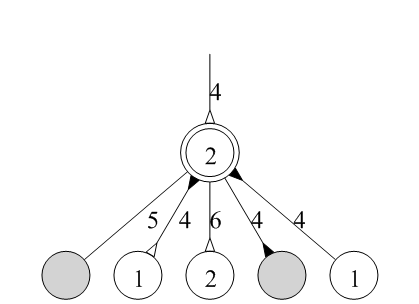
\includegraphics[width=.35\linewidth]{segmentation-waterfall-smg-pass1cases-d.png}\hspace{8mm}}%
	%
	\hspace{4mm}%
	%
	\subfigure[There is no flow out of the node]
	{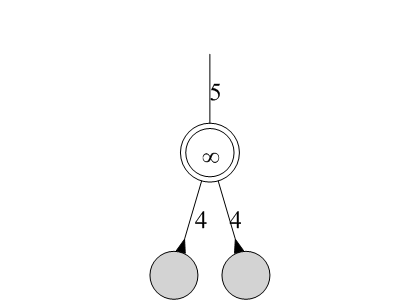
\includegraphics[width=.35\linewidth]{segmentation-waterfall-smg-pass1cases-e.png}}%
	%
	\hspace{4mm}%
	%
	\subfigure[There is no downwards flow out of the node (but the parent edge still needs to be considered)]
	{\hspace{8mm}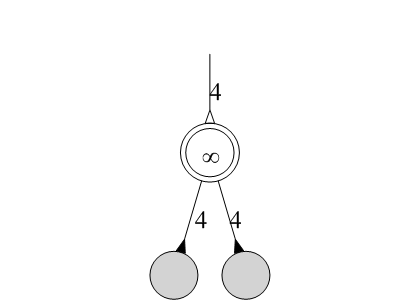
\includegraphics[width=.35\linewidth]{segmentation-waterfall-smg-pass1cases-f.png}\hspace{8mm}}%
\caption{Case analysis for the first pass of my waterfall algorithm}
\label{fig:segmentation-waterfall-smg-pass1cases}
\end{stusubfig}
%---

%---
\begin{stusubfig}{p}
	\subfigure[The arrow from the parent node points towards us]
	{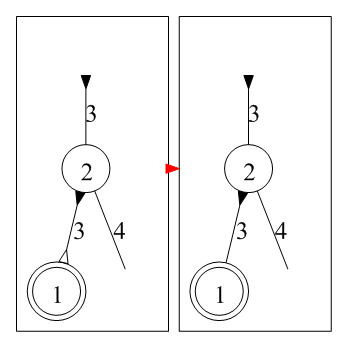
\includegraphics[height=5.5cm]{segmentation-waterfall-smg-resolutioncases-a.png}}%
	%
	\hspace{4mm}%
	%
	\subfigure[There is no flow from the parent node]
	{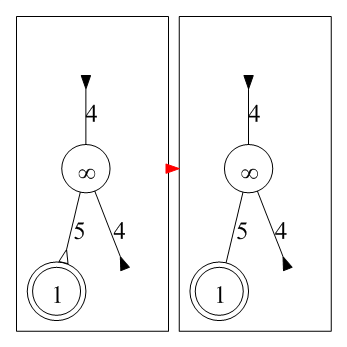
\includegraphics[height=5.5cm]{segmentation-waterfall-smg-resolutioncases-b.png}}%
	%
	\hspace{4mm}%
	%
	\subfigure[There is an equally good route via the parent node]
	{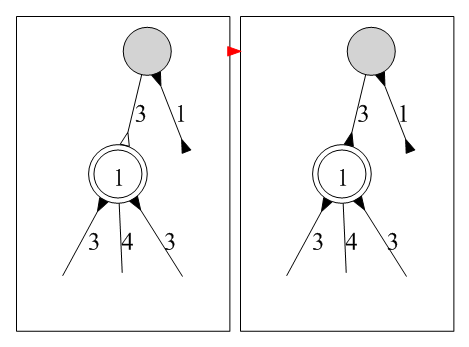
\includegraphics[height=5.5cm]{segmentation-waterfall-smg-resolutioncases-c.png}}%
	%
	\hspace{4mm}%
	%
	\subfigure[There is a better route via the parent node]
	{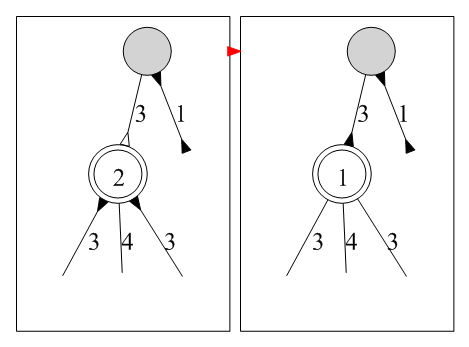
\includegraphics[height=5.5cm]{segmentation-waterfall-smg-resolutioncases-d.png}}%
\caption[Case analysis for the resolution step of my waterfall algorithm]{Case analysis for the resolution step of my waterfall algorithm (the circled node is the one currently under consideration in each case)}
\label{fig:segmentation-waterfall-smg-resolutioncases}
\end{stusubfig}
%---

%---
\begin{stusubfig}{p}
	\subfigure[The initial tree]{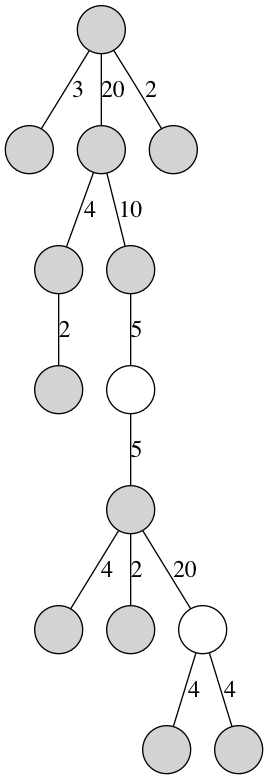
\includegraphics[width=.3\linewidth]{segmentation-waterfall-smg-example-initial.png}}%
	\hspace{4mm}%
	\subfigure[After the first pass]{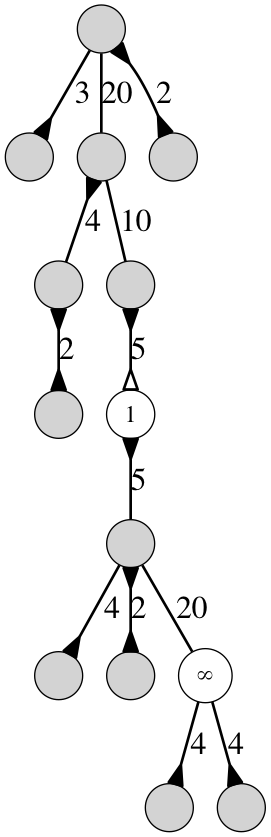
\includegraphics[width=.3\linewidth]{segmentation-waterfall-smg-example-pass1.png}}%
	\hspace{4mm}%
	\subfigure[After the second pass]{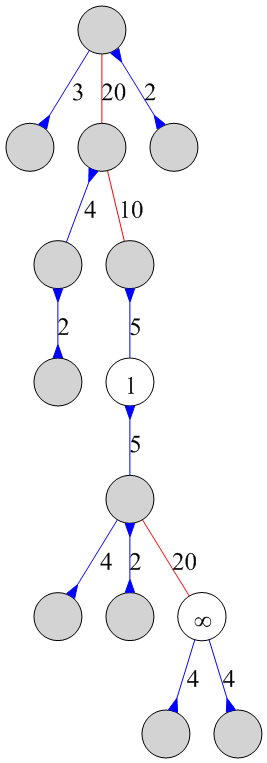
\includegraphics[width=.3\linewidth]{segmentation-waterfall-smg-example-pass2.png}}%
\caption[My waterfall algorithm running on a real example]{My waterfall algorithm running on a real example: the arrows on the nodes indicate the flow direction, blue edges are those that will be elided and red edges are those that won't be.}
\label{fig:segmentation-waterfall-smg-example}
\end{stusubfig}
%---

\bibliographystyle{alpha}
\bibliography{existingwork,mypapers}

\end{document}
